\chapter{L'azienda Digicando}
\label{lazienda-digicando}
L'azienda Digicando viene fondata nel 2015, con lo scopo di aiutare i brand a proteggersi dalla contraffazione e, allo stesso tempo, aiutarli a conoscere meglio i loro target di utenti attraverso l'analisi di big data. L'azienda offre servizi di tracciabilità, anticontraffazione ed analisi statistica sugli acquirenti dei prodotti. Attualmente la piattaforma si basa su un'infrastruttura classica di tipo client-server, ma l'obiettivo è la decentralizzazione graduale del servizio mediante la tecnologia \emph{blockchain}, con lo scopo di ottenere un sistema completamente \emph{trustless}, quindi senza necessità di fiducia tra le varie parti nelle sue funzionalità di base, con una gestione trasparente e sicura dei dati. Con l'implementazione attuale, la veridicità delle informazioni ricavate dal servizio deriva dalla fiducia dell'utente finale verso il produttore e sulla gestione dei dati da parte di Digicando.

\section{Problema}
\label{problema}
Il servizio di Digicando mira a risolvere una serie di problematiche, che si possono riassumere come segue:
\begin{itemize}
    \item Attualmente non è possibile verificare le specifiche complete di un prodotto, ma ci si deve fidare di ciò che c'è scritto sull'etichetta. Generalmente, non è possibile determinare la qualità di un oggetto in vendita, online ed in un negozio fisico, e la genuinità delle relative recensioni.
    \item Le procedure di attivazione della garanzia sono costose e spesso inutilizzate dai clienti; inoltre, le ricevute di acquisto, essendo stampate su carta termica, sono soggette ad un rapido deterioramento con conseguente impossibilità di far valere il diritto alla garanzia.
    \item I produttori utilizzano sistemi spesso poco efficaci per tracciare e controllare il lavoro degli esterni e dei venditori.
    \item I prodotti contraffatti vengono venduti nei negozi, compromettendo i guadagni e l'immagine dei produttori. Per identificare i prodotti contraffatti i produttori spendono milioni di euro all'anno in investigazioni.
\end{itemize}

\subsection{La contraffazione}
\label{la-contraffazione}
Secondo una ricerca dell'EUIPO, all'interno dell'Unione Europea la contraffazione costa ogni anno 60 miliardi di euro in 13 settori economici, pari a 116 euro pro capite. Tale valore delle perdite, causato dalla presenza di prodotti falsi sul mercato, è pari al 7.5\% delle rispettive vendite. In Italia la situazione è ancora peggiore, con perdite annue pari al 7.9\% delle vendite dirette, per un valore complessivo di 8.6 miliardi di euro \cite{euipo}.

La produzione di merci contraffatte è in aumento e, anche se viene considerato un fenomeno esterno all'Unione Europea, risulta visibile anche al suo interno. La contraffazione, insieme alla pirateria, causerebbe la perdita di circa 800.000 posti di lavoro \cite{eesc}.

\section{Soluzione}
\label{soluzione}
La soluzione ai problemi sopra elencati è la creazione di un sistema che garantisca l'originalità di un prodotto con certezza e che assicuri l'acquisto dell'utente finale. \emph{bCerty} è il servizio che fornisce ai clienti la certificazione sia dell'originalità dei prodotti che del loro postvendita. Il sistema permette anche la certificazione di proprietà di ogni oggetto e la gestione della sua garanzia.

Il servizio di Digicando è basato su \emph{tag} unici applicati al prodotto che sfruttano un sistema di algoritmi brevettato per la verifica dell'originalità. I tag possono essere microchip NFC oppure etichette con un codice esposto, generalmente un QR-code, ed uno nascosto e svelabile con un'azione meccanica.


\section{Implementazione client-server}
\label{implementazione-client-server}
L'applicazione client-server attuale è basata sul cloud ed espone delle \emph{API (Application Programming Interface)} ed un portale web per accedere al servizio. L'applicazione server è scritta per il framework multipiattaforma ASP.NET core ed è stata sviluppata seguendo l'approccio \emph{Domain-Driven Design}, che prevede l'organizzazione dell'architettura in tre livelli:
\begin{itemize}
    \item \emph{Dominio}: contiene i modelli, i servizi a loro associati e le logiche delle operazioni complesse, come per esempio l'emissione di un ordine di produzione di tag da parte di un produttore.
    \item \emph{Infrastruttura}: contiene il database, l'\emph{Object Data Manager (ODM)} ed i servizi esterni, come per esempio i servizi di comunicazione con la blockchain che sono attualmente in fase di sviluppo e test.
    \item \emph{Applicativo}: contiene le applicazioni che utilizzano il dominio, tra cui la \emph{Web App}, le \emph{API} e tutti i processi in background, come per esempio  il processo di creazione dei tag. Questo livello attualmente implementa anche i sistemi di sicurezza e autorizzazione per l'accesso ai dati, con il rischio che un errore di programmazione esponga dati sensibili a persone non autorizzate. Per questo motivo la parte di sicurezza ed autorizzazione verrà spostata a livello di dominio.
\end{itemize}

Il portale web consiste di una parte dedicata agli utenti finali, cioè i consumatori, e di un pannello per la gestione della produzione dedicato agli operatori dei brand, dove è possibile amministrare gli articoli ed i tag per i loro prodotti.

Sono state sviluppate anche delle applicazioni per i consumatori, destinate alle piattaforme più popolari: Windows, iOS ed Android. Queste applicazioni sono sviluppate sincronicamente grazie al framework \emph{Xamarin} e riproducono gli aspetti del portale web dedicato ai consumatori, con l'aggiunta di funzioni che richiedono l'accesso all'hardware dei dispositivi, come l'NFC per la verifica dell'originalità.

Infine, è stata sviluppata un'applicazione desktop per Windows dedicata ai brand, per la gestione della produzione. Con questa applicazione è possibile scansionare i tag di produzione, attivarli e stampare le etichette. In futuro, quest'applicazione sarà resa compatibile anche con macOS e Linux.

\paragraph{Database}
\label{database}
L'applicazione utilizza un database documentale \emph{MongoDB}, per il quale è stato sviluppato da Digicando un Object Data Manager in ambiente .NET che ne rende più agile la gestione. Questo ODM serve a ridurre le query al database e a migliorare le interconnessioni tra documenti. Implementa un complesso meccanismo di \emph{caching} che mantiene in memoria i documenti usati recentemente. La cache mantiene i documenti letti direttamente, ma anche quelli letti da riferimenti contenuti in altri documenti. Basandosi sull'assunzione che le letture nel database sono più frequenti delle scritture, è conveniente denormalizzare i dati. La denormalizzazione rischia però di portare ad inconsistenze. Questo problema è stato risolto sviluppando un sistema che lavora in \emph{background} e modifica automaticamente tutti i riferimenti ad un documento quando esso viene modificato. È previsto che il codice sorgente dell'ODM venga rilasciato liberamente.

Attualmente nel database vengono memorizzati tutti i dati, tra cui i tag, le informazioni riguardanti i produttori, gli utenti ed i loro ruoli, le verifiche e le scansioni.

\section{Implementazione con blockchain}
\label{implementazione-con-blockchain}
L'obiettivo di Digicando è spostare il servizio di identificazione univoca di ogni singolo oggetto e la sua proprietà su blockchain. Il risultato finale sarà quindi un sistema ibrido tra blockchain e client-server.

L'implementazione con blockchain prevede l'applicazione di marcatori univoci, chiamati \emph{tag}, sui prodotti su cui sia scritto fisicamente l'indirizzo di un token digitale mediante un QR-code, tag NFC o altre soluzioni. Sono attualmente in fase di studio e progettazione altri speciali marcatori che combinino tecnologie più avanzate per la protezione di prodotti più costosi. Risulta importante mantenere un basso costo per i marcatori, per non impattare negativamente sul costo del prodotto stesso. L'esempio più semplice di marcatore fisico è un'etichetta.

\subsection{Motivazioni}
\label{motivazioni}
L'utilizzo della tecnologia blockchain fornisce un'infrastruttura che registra, certifica e mappa i trasferimenti di una proprietà tra parti spesso distanti. In questo modo è possibile mantenere la cronologia di trasferimenti nella catena di distribuzione di un prodotto, in maniera immodificabile, sicura, trasparente ed aperta al controllo di chiunque o di utenti autorizzati.

\subsection{Architettura}
L'architettura del sistema è suddivisa in livelli:
\begin{itemize}
    \item \emph{Identity service}: un sistema per identificare gli operatori, che definisce gli indirizzi che possono operare sulla blockchain, con una gestione dei loro ruoli e dei permessi. Questo sistema sarà utilizzato come base per identificare i produttori, i venditori e i loro delegati.
    \item \emph{Item manager}: si occupa della gestione, della produzione, dell'acquisto, dello scambio e della verifica dei tag.
    \item \emph{Social application}: permette agli utenti di fare valutazioni ed osservazioni sui prodotti, di pubblicare materiale correlato ai prodotti in spazi privati e di organizzare vendite protette. Questo layer verrà decentralizzato solo in un secondo momento.
    \item \emph{Managed services}: consiste di un'applicazione server che fornisce i servizi e le API non decentralizzati. Questo layer non fornisce funzionalità di base, ma solo l'accesso ai dati ed ai servizi. Rende inoltre possibile la gestione ed il processo dei dati che, per varie ragioni, si preferisce non decentralizzare.
    \item \emph{Client}: raccoglie le applicazioni ed il portale web che fungono da \emph{entry-point} per l'esperienza utente. Questo livello si interfaccia con i nodi della blockchain e le API server \cite{bCerty-whitepaper}.
\end{itemize}

\begin{figure}[h!]
    \centering
    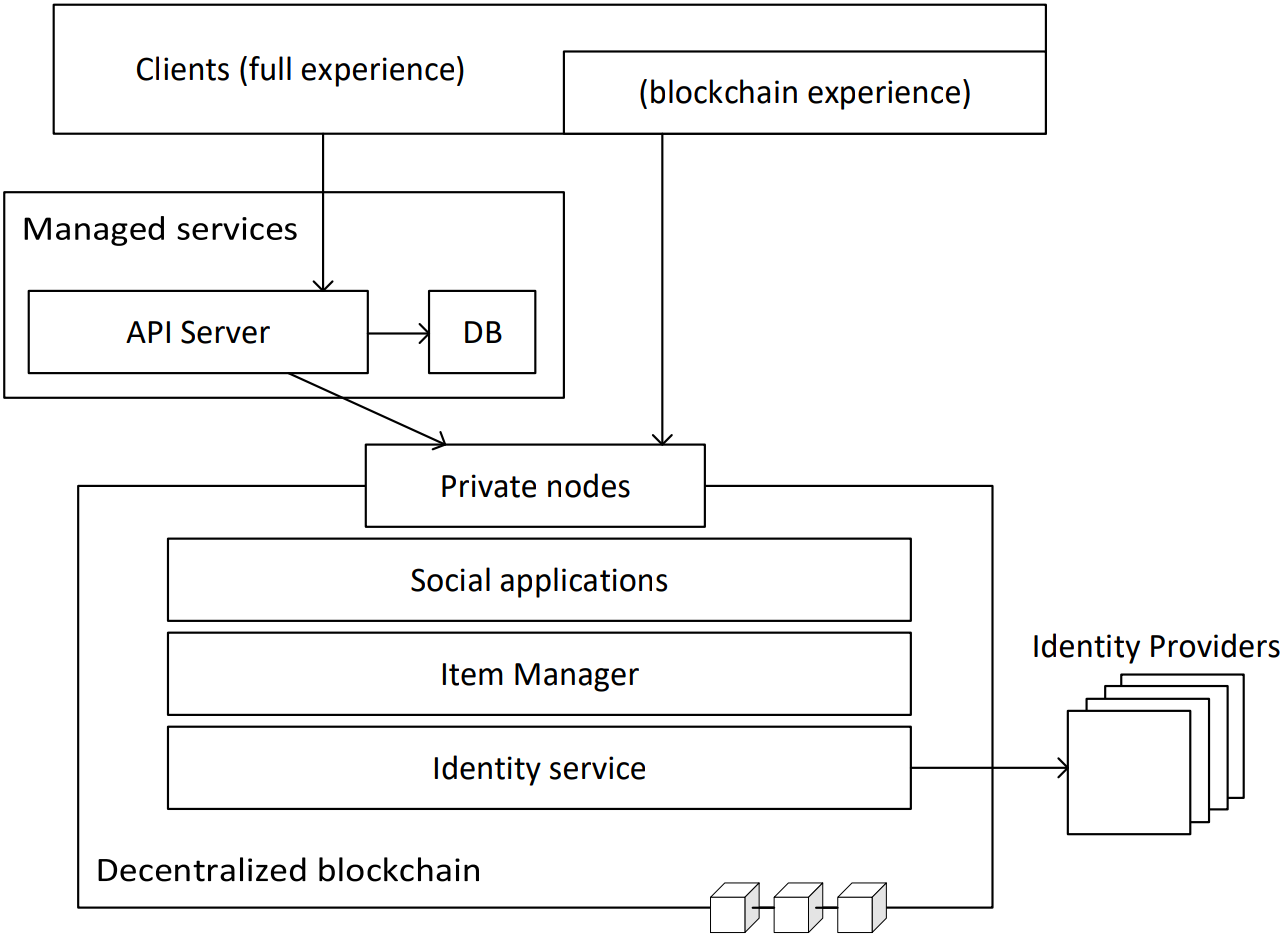
\includegraphics[scale=0.25]{img/architettura.png}
    \caption{Architettura dell'implementazione con blockchain}
    \label{fig:architettura}
\end{figure}

\subsection{Tag}
\label{tag}
Ogni tag ha un identificativo univoco che permette di identificare l'oggetto fisico o virtuale che rappresentano del quale un utente può detenere la proprietà. I tag vengono creati da un contratto, che li emette sotto forma di token non fungibili, compatibili con lo standard \emph{ERC721}. I token sono corredati da un identificativo pubblico e da eventuali chiavi private. Le chiavi private possono servire a sbloccare la proprietà del token in fase di acquisto del prodotto, oppure per la verifica dell'autenticità.
I tag possono essere di due tipi:
\begin{itemize}
    \item \emph{Personal tag}: possono essere prodotti da qualsiasi utente senza particolari requisiti e possono essere garantiti dall'utente stesso attraverso mezzi indipendenti. Sono dedicati alla catalogazione di beni personali per l'uso privato. Contengono direttamente le informazioni dell'oggetto che possono essere crittografate.
    \item \emph{Production tag}: sono destinati alla produzione di massa. Sono collegati ad un produttore e possono essere identificati come genuini se il produttore ha un certificato valido. Questi tag sono associati ad un profilo oggetto contenente le informazioni dell'oggetto stesso, che può essere modificato solamente dal produttore o dai suoi delegati. Questi tag possono essere abilitati per l'acquisto, per la verifica e possono contenere un premio di verifica.
\end{itemize}

I tag possono essere creati direttamente già attivati, oppure essere attivati successivamente dal produttore o da un venditore autorizzato. Un tag non attivo è un tag che non viene più riconosciuto dal produttore e che quindi non è più accessibile e verificabile. Se un tag è attivo può essere acquistato autonomamente da un utente finale.

I tag possono essere acquistati autonomamente da un produttore in ether tramite un contratto, oppure il produttore può rivolgersi a Digicando per pagare in altre valute. Il costo di un tag è definito arbitrariamente da bCerty, osservando il valore dell'ether nel mercato ed aggiornandolo periodicamente di conseguenza \cite{bCerty-whitepaper}.

\subsection{Verifica di un prodotto}
\label{verifica-di-un-prodotto}
Il servizio su blockchain prevede la possibilità per ogni utente di verificare l'autenticità di un prodotto tramite lo \emph{smartphone} senza la necessità di procedere con l'acquisto, ricevendo una ricompensa. Ad ogni prodotto, o lotto di prodotti, può essere infatti associato un premio, chiamato \emph{bounty}, correlato a diverse operazioni che l'utente può compiere: acquisto, verifica dell'originalità del token, scambio di oggetti tra utenti. Insieme alla conferma di originalità l'utente può ricevere delle informazioni riguardanti il prodotto. Questo processo di verifica con ricompensa permette di ottenere un controllo di anticontraffazione distribuito, senza la necessità per il produttore di organizzare esso stesso i controlli, e rende ogni utente un potenziale investigatore privato.

Ogni tag verificabile è fornito di un tag NFC leggibile e scrivibile, nel quale viene memorizzato un codice dinamico. Il codice è una chiave di crittografia privata ellittica di cui è possibile trovare la chiave pubblica corrispondente tramite la blockchain associata al tag. Se le chiavi corrispondono il tag è originale. Il sistema prevede che il codice sia aggiornato per prevenire la creazione di cloni dello stesso tag. L'aggiornamento del codice dinamico non è obbligatorio, ma il produttore può impostare dei criteri per premiare chi decide di farlo, per esempio i \emph{bounty} di verifica. Ogni operazione di verifica è tracciata sulla blockchain, fatta eccezione per le verifiche negative che innescano opzionalmente l'invio al sistema di un rapporto contenente tutti i dati necessari per comprendere l'accaduto \cite{bCerty-whitepaper}.

\paragraph{Bounty di verifica}
Ogni tag contiene un bounty di verifica, impostato dal produttore ed espresso in ether. Il bounty viene rilasciato quando il prodotto viene acquistato, distribuendolo a tutti coloro che hanno verificato l'originalità del prodotto e hanno aggiornato correttamente il codice. Il bounty viene distribuito proporzionalmente ai lassi di tempo intercorsi tra le diverse verifiche, per evitare che uno stesso utente compia diverse verifiche con diversi indirizzi per aggiudicarsi un bounty più grande.

Il produttore può prestabilire il momento di attivazione del bounty, per esempio attivandolo all'arrivo in negozio, per evitare che gli addetti al trasporto possano aggiudicarsi un bounty o che il primo verificatore si aggiudichi il bounty relativo a tutto il tempo di trasporto. In alternativa il venditore del negozio può essere incaricato dal produttore di controllare ed attivare i tag dei prodotti che riceve.

\subsection{Acquisto}
\label{acquisto}
L'acquisto viene eseguito tramite una chiave segreta stampata sul tag tramite un codice, generalmente di tipo QR. Questo codice può essere scoperto solo tramite un'azione meccanica irreversibile sul tag ed è necessario per effettuare una transazione che firma l'indirizzo dell'acquirente tramite la chiave trovata. Un contratto su blockchain verificherà poi la firma utilizzando la chiave pubblica e verificherà che l'indirizzo mostrato corrisponda al nome dell'acquirente; se corrisponde la vendita sarà autorizzata.

\subsection{Scambio e rivendita di prodotti usati}
Utilizzando un contratto specifico è possibile rivendere prodotti usati. Il contratto certifica il possesso dell'oggetto da parte del venditore e raccoglie il pagamento del compratore. Solamente quando entrambe le parti avranno completato con successo le transazioni il contratto rilascerà il credito al venditore e trasferirà il possesso al compratore. Le vendite possono essere effettuate in ether, oppure in altre valute regolate da un oracolo. 

\subsection{Memorizzazione dei dati}
Tutti i dati di grandi dimensioni e non critici dal punto di vista della privacy verranno memorizzati su IPFS o Swarm. Questi dati comprendono:
\begin{itemize}
    \item I dati multimediali.
    \item Le descrizioni testuali di prodotti, produttori, utenti ed altro.
    \item I commenti riguardanti la qualità dei prodotti e le recensioni.
\end{itemize}

I dati funzionali invece, verranno memorizzati direttamente sulla blockchain all'interno dei contratti. Questi dati comprendono, per esempio, le chiavi di sblocco dei prodotti.

Per garantire la protezione della privacy alcuni dati di servizio saranno mantenuti privati da Digicando e non saranno pubblicati sulla blockchain; questi comprendono le informazioni personali degli utenti e dei produttori, le analisi di utilizzo dell'applicazione, le informazioni riguardanti le verifiche e le letture dei tag e gli oggetti che non hanno la certificazione bCerty.

\subsection{Adozione del servizio basato su blockchain}
\label{adozione-del-servizio-basato-su-blockchain}
La transizione al servizio basato su blockchain sarà graduale e, almeno inizialmente, facoltativa, per rendere questo processo il meno problematico possibile per tutte le parti interessate. Inizialmente l'implementazione su blockchain verrà distribuita sulla \emph{testnet Ropsten} ed utilizzata unicamente per un \emph{beta testing} interno. Seguirà una fase dove le due implementazioni coesisteranno. Solamente in un secondo momento, quando il servizio su blockchain sarà completamente funzionante ed ampiamente testato, si procederà con lo spegnimento dei server non più utili al funzionamento.

\subsection{Svantaggi e considerazioni sull'utilizzo della blockchain}
\label{svantaggi-e-considerazioni}
La transizione ad un servizio basato su blockchain porta una serie di svantaggi e di problematiche da risolvere: primo fra tutti la mancanza del concetto di segretezza; ogni dato pubblicato su blockchain infatti non sarà mai completamente privato. Questo problema ha portato a varie difficoltà nell'implementazione dell'algoritmo di verifica con chiavi segrete dinamiche brevettato da Digicando, che è stato quindi modificato. Una seconda problematica, non direttamente collegata a Digicando, è la scalabilità della blockchain. Il numero di transazioni che la rete è in grado di gestire in un'unità di tempo è limitato e, attualmente, particolarmente basso. Con l'aumento degli utilizzatori della rete questo problema non può che peggiorare. In futuro si pensa di migrare il servizio su una blockchain Plasma, per risolvere questo problema. Una terza problematica infine, può essere la futura promulgazione di leggi che limitino le possibilità di utilizzo e l'adozione della tecnologia blockchain.

\newpage